\part{Python}

\chapter{Базовый понятия}

\section{Стандартные типы}

	К стандартным типам данных в Python относят:
	\begin{itemize}
		\item Числа: целые (int), вещественные (float), комплексные (complex);
		\item Байты (bytes и bytearray);
		\item Множества (set и frozenset);
		\item Кортежи (tuple) и Списки (list);
		\item Строки (str);
		\item Исключения (exceptions);
		\item None.
	\end{itemize}
	
\section{Разница между списками и котежами, когда используются}

	Списки в Python - упорядоченные изменяемые коллекции объектов произвольных типов.  
Кортеж — это неизменяемый список. С момента создания кортеж не может быть изменен никакими способами.  Кортеж определяется так же, как и список, но элементы перечисляются в круглых скобках вместо квадратных.
	\begin{itemize}
\item	Как и в списках, элементы в кортежах имеют определенный порядок. Точно так же нумерация элементов начинается с нуля. 
\item	Как и для списков, отрицательные индексы позволяют вести отсчет элементов с конца кортежа.
\item	К кортежам, как и к спискам можно применить операцию среза. Обратите внимание, что срез списка — новый список, а срез кортежа — новый кортеж.
\item	Работа с кортежами быстрее, чем со списками. Если вы определяете постоянный набор значений, и все, что вы хотите с ним когда-либо делать, это перебирать его элементы, используйте кортеж вместо списка.
\item	Кортеж может быть преобразован в список и наоборот.
	\end{itemize}
	
\section{Стандартные библиотеки python, работа с датами, регулярными выражениями}

Стандартные библиотеки python, работа с датами, регулярными выражениями

		\begin{itemize}
	
		\item unittest - поддерживает автоматизацию тестов, использование общего кода для настройки и завершения тестов, объединение тестов в группы, а также позволяет отделять тесты от фреймворка для вывода информации.
		\item subprocess - отвечает за выполнение следующих действий: порождение новых процессов, соединение c потоками стандартного ввода, стандартного вывода, стандартного вывода сообщений об ошибках и получение кодов возврата от этих процессов.
		\item fractions - предоставляет поддержку рациональных чисел.
		\item cmath – предоставляет функции для работы с комплексными числами.
		\item copy - поверхностное и глубокое копирование объектов.
		\item os.path - является вложенным модулем в модуль os, и реализует некоторые полезные функции на работы с путями.
		\item json - позволяет кодировать и декодировать данные в удобном формате. JSON (JavaScript Object Notation) - простой формат обмена данными, основанный на подмножестве синтаксиса JavaScript.
		\item calendar - позволяет напечатать себе календарик (а также содержит некоторые другие полезные функции для работы с календарями).
		\item os - предоставляет множество функций для работы с операционной системой, причём их поведение, как правило, не зависит от ОС, поэтому программы остаются переносимыми.
		\item pickle - реализует мощный алгоритм сериализации и десериализации объектов Python. "Pickling" - процесс преобразования объекта Python в поток байтов, а "unpickling" - обратная операция, в результате которой поток байтов преобразуется обратно в Python-объект. Так как поток байтов легко можно записать в файл, модуль pickle широко применяется для сохранения и загрузки сложных объектов в Python.
		\item datetime - предоставляет классы для обработки времени и даты разными способами. Поддерживается и стандартный способ представления времени, однако больший упор сделан на простоту манипулирования датой, временем и их частями.
		\item array - определяет массивы в python. Массивы очень похожи на списки, но с ограничением на тип данных и размер каждого элемента.
		\item Time - модуль для работы со временем в Python.
		\item. sys - обеспечивает доступ к некоторым переменным и функциям, взаимодействующим с интерпретатором python.
		\item math – один из наиважнейших в Python. Этот модуль предоставляет обширный функционал для работы с числами.
		\item регулярное выражение — это последовательность символов, используемая для поиска и замены текста в строке или файле. В Python для работы с регулярными выражениями есть модуль re. Регулярные выражения используют два типа символов: специальные символы: как следует из названия, у этих символов есть специальные значения, например, * означает «любой символ»; литералы (например: a, b, 1, 2 и т. д.).
	\end{itemize}

\section{Что такое PEP8}

python enhanced proposal — заявки на улучшение языка python), описывающий, какого стиля следует придерживаться при написании кода на C в реализации языка python

\section{Сделать свапинг 2х переменных}	

Сделать свапинг 2х переменных
	\begin{python}
		x=1
		y=2
		x,y=y,x
	\end{python}

\section{min(), max(), sorted()}

	min() max()

		В языке программирования Python есть встроенные функции поиска минимума и максимума. Им можно передавать как один объект (список или другой объект-последовательность или итерируемый объект), так и непосредственно множество однотипных объектов. Если передается один список, то в нем находится минимум или максимум, который возвращается.
	\begin{python}
		>>> a = [45, 56, 12] 
		>>> min(a) 
		12 
	\end{python}
	\begin{itemize}
			
		\item Если передается несколько списков, то возвращается целый список. При этом сравнение происходит поэлементно: сначала сравниваются первые элементы списков. Если они не равны, то функция min вернет тот список, первый элемент которого меньше (max наоборот). Если первые элементы равны, то будут сравниваться вторые и т. д.
		\begin{python}
>>> b = [89, 0, 11] 
>>> min(a,b) 
45, 56, 12
		\end{python}
		\item В функциях min и max можно указать необязательный именной параметр key. Ему присваивается одноаргументная функция, которая выполняет какое-то предварительное действие над элементами, например, списка.
		\item Однако нельзя передать или смешанный список.	
	\end{itemize}
		
\section{Дается строка, разрезать по разделителю}

	Дается строка, разрезать по разделителю. Почтитать про операции со строками
	
	\begin{itemize}
	
		\item Базовые операции
		Конкатенация (сложение) S1 + S2, Дублирование строки 'spam' * 3, Длина строки (функция len), Доступ по индексу S[0], Извлечение среза s[3:5], Кроме того, можно задать шаг, с которым нужно извлекать срез s[3:5:1]. 
		\item S.split(символ)	Разбиение строки по разделителю
		\item S.find(str, [start],[end])	Поиск подстроки в строке. Возвращает номер первого вхождения или -1
		\item S.join(список)	Сборка строки из списка с разделителем S
		\item S.center(width, [fill])	Возвращает отцентрованную строку, по краям которой стоит символ fill (пробел по умолчанию)
		\item S.strip([chars])	Удаление пробельных символов в начале и в конце строки
		\item Форматирование строк с помощью метода format:
		\begin{python}
			>>> '{0}, {1}, {2}'.format('a', 'b', 'c')
			'a, b, c'
		\end{python}
	\end{itemize}

\section{Все мьютебл (изменяемые) и не мьютебл типы}

Все типы данных в Python относятся к одной из 2-х категорий: изменяемые (mutable) и неизменяемые (unmutable)( immutable). Многие из предопределённых типов данных Python — это типы неизменяемых объектов: числовые данные (int, float, complex), символьные строки (class 'str'), кортежи (tuple). Другие типы определены как изменяемые: списки (list), множества (set), словари (dict). Вновь определяемые пользователем типы (классы) могут быть определены как неизменяемые или изменяемые. Изменяемость объектов определённого типа является принципиально важной характеристикой, определяющей, может ли объект такого типа выступать в качестве ключа для словарей (dict) или нет.
Immutable типы в Python — это числа(numbers), строки (strings) и кортежи (tuples).	

\section{Менеджер контекста}		

Менеджер контекста. Что это такое, зачем, для чего применяются, чем можно заменить. 

		Контекстные менеджеры это специальные конструкции, которые представляют из себя блоки кода, заключенные в инструкцию with. Из этого следует, что контекстный менеджер используется для выполнения каких либо действий до входа в блок и после выхода из него.  Применяется для гарантии того, что критические функции выполнятся в любом случае. Самый распространённый пример использования этой конструкции - открытие файлов. Аналог - открытии файлов с помощью функции open, однако конструкция with ... as, как правило, является более удобной и гарантирует закрытие файла в любом случае.
	
	Общий вид: Конструкция with ... as используется для оборачивания выполнения блока инструкций менеджером контекста. Иногда это более удобная конструкция, чем try...except...finally.
	\begin{python}
	"with" expression ["as" target] ("," expression ["as" target])* ":"
	    suite
	\end{python}
	
	Теперь по порядку о том, что происходит при выполнении данного блока:
	\begin{itemize}
		\item Выполняется выражение в конструкции with ... as.
		\item Загружается специальный метод \pyth{__exit__} для дальнейшего использования.
		\item Выполняется метод \pyth{__enter__}. Если конструкция with включает в себя слово as, то возвращаемое методом \pyth{__enter__} значение записывается в переменную.
		\item Выполняется suite.
		\item Вызывается метод \pyth{__exit__}, причём неважно, выполнилось ли suite или произошло исключение. В этот метод передаются параметры исключения, если оно произошло, или во всех аргументах значение None, если исключения не было.
	\end{itemize}
	
	Пример собственного контекстного менеджера:
	\begin{python}
			class Hello:
	   ...:     def __del__(self):
	   ...:         print u'destructor'
	   ...:     def __enter__(self):
	   ...:         print u'enter to block'
	   ...:     def __exit__(self, exp_type, exp_value, traceback):
	   ...:         print u'exit from block'
	\end{python}
	
\section{Итераторы, генераторы. Yield}

\textit{Итераторы}

Для понимания, что делает yield, необходимо понимать, что такое генераторы. Генераторам же предшествуют итераторы. Когда вы создаёте список, вы можете считывать его элементы один за другим — это называется итерацией:

\begin{python}
>>> mylist = [1, 2, 3]
>>> for i in mylist :
...    print(i)
1
2
3
\end{python}

Mylist является итерируемым объектом. Когда вы создаёте список, используя генераторное выражение, вы создаёте также итератор:

\begin{python}
>>> mylist = [x*x for x in range(3)]
>>> for i in mylist :
...    print(i)
0
1
4
\end{python}

Всё, к чему можно применить конструкцию «for… in...», является итерируемым объектом: списки, строки, файлы… Это удобно, потому что можно считывать из них значения сколько потребуется — однако все значения хранятся в памяти, а это не всегда желательно, если у вас много значений.

\textit{Генераторы}

Генераторы это тоже итерируемые объекты, но прочитать их можно лишь один раз. Это связано с тем, что они не хранят значения в памяти, а генерируют их на лету:

\begin{python}
>>> mygenerator = (x*x for x in range(3))
>>> for i in mygenerator :
...    print(i)
0
1
4
\end{python}

Всё то же самое, разве что используются круглые скобки вместо квадратных. НО: нельзя применить конструкцию for i in mygenerator второй раз, так как генератор может быть использован только единожды: он вычисляет 0, потом забывает про него и вычисляет 1, завершаяя вычислением 4 — одно за другим.

\textit{Yield}

Yield это ключевое слово, которое используется примерно как return — отличие в том, что функция вернёт генератор.

\begin{python}
>>> def createGenerator() :
...    mylist = range(3)
...    for i in mylist :
...        yield i*i
...
>>> mygenerator = createGenerator() # create generator
>>> print(mygenerator) # mygenerator is object!
<generator object createGenerator at 0xb7555c34>
>>> for i in mygenerator:
...     print(i)
0
1
4
\end{python}

В данном случае пример бесполезный, но это удобно, если вы знаете, что функция вернёт большой набор значений, который надо будет прочитать только один раз.
Чтобы освоить yield, вы должны понимать, что когда вы вызываете функцию, код внутри тела функции не исполняется. Функция только возвращает объект-генератор — немного мудрёно :-)
Ваш код будет вызываться каждый раз, когда for обращается к генератору.
В первый запуск вашей функции, она будет исполняться от начала до того момента, когда она наткнётся на yield — тогда она вернёт первое значение из цикла. На каждый следующий вызов будет происходить ещё одна итерация написанного вами цикла, возвращаться будет следующее значение — и так пока значения не кончатся.
Генератор считается пустым, как только при исполнении кода функции не встречается yield. Это может случиться из-за конца цикла, или же если не выполняется какое-то из условий «if/else».

\textit{Итератор} — это объект-абстракция, который позволяет брать из источника, будь это stdin или, скажем, какой-то большой контейнер, элемент за элементом, при этом итератор знает только о том объекте, на котором он в текущий момент остановился.
В Python (и не только в нем) есть два понятия, которые звучат практически одинаково, но обозначают разные вещи, — iterator и iterable. Первое — это объект, который реализует описанный выше интерфейс, а второе — контейнер, который может служить источником данных для итератора.
Если простым языком, генераторное выражение — это еще один синтаксический сахар в Python, простейший способ создать объект с интерфейсом итератора, при этом не загружая всех элементов в память (а это чаще всего и не нужно).
Основная фишка генератора в том, что он, подобно итератору, запоминает последний момент, когда к нему обращались, но при этом оперирует не абстрактными элементами, а вполне конкретными блоками кода. То есть если итератор по умолчанию будет перебирать элементы в контейнере, пока они не кончатся, то генератор будет гонять код, пока не выполнится какое-нибудь конкретное условие возврата. 

\textit{итератор:}
\begin{python}
class SimpleIterator(object):
 2     
 3     def __init__(self,fname):
 4         self.fd = open(fname,'r')
 5         
 6     def __iter__(self):
 7         return self
 8 
 9     def next(self):
10         l = self.fd.readline()
11         if l != '':
12             l = l.rstrip('\n')
13             num = int(l)
14             return num*2
15         raise StopIteration
\end{python}

\textit{генератор:}
\begin{python}
1 def power(start):
2     print "power is called the first time"
3     for i in xrange(start,start+5):
4         yield i*i
5     print "power is called the last time"
\end{python}

\section{lambda или анонимные функции}		

Анонимные функции не имеют имени и состоят из единственного выражения, значение которого является возвращаемым значением функции. Анонимные функции создаются с помощью ключевого слова lambda и используется в виде: lambda <аргументы>: <выражение> . Их удобно использовать для создания небольших функций. Анонимные функции являются выражением, в отличие от инструкции def. Вследствие этой особенности, lambda-выражения можно использовать в тех участках кода, где нельзя использовать def. Анонимные функции можно присваивать переменным.

Анонимные функции создаются с помощью инструкции lambda. Кроме этого, их не обязательно присваивать переменной, как делали мы инструкцией def func():
\begin{python}
>>>
>>> func = lambda x, y: x + y
>>> func(1, 2)
3
>>> func('a', 'b')
'ab'
>>> (lambda x, y: x + y)(1, 2)
3
>>> (lambda x, y: x + y)('a', 'b')
'ab'
>>>
>>> func = lambda *args: args
>>> func(1, 2, 3, 4)
(1, 2, 3, 4)
>>> a=[lambda x:x, lambda x:2*x]
>>> for i in a: print i(2)
... 
2
4
>>> func=lambda a,b:a+b
>>> func(1,2)
3	
\end{python}

\section{ООП. Метод класса и статический метод}

Принципы ООП

\begin{itemize}
\item Абстракция данных - Абстрагирование означает выделение значимой информации и исключение из рассмотрения незначимой. 
\item Инкапсуляция — свойство системы, позволяющее объединить данные и методы, работающие с ними, в классе.
\item Наследование — свойство системы, позволяющее описать новый класс на основе уже существующего с частично или полностью заимствующейся функциональностью. Класс, от которого производится наследование, называется базовым, родительским или суперклассом. Новый класс — потомком, наследником, дочерним или производным классом.
\item Полиморфизм подтипов (в ООП называемый просто «полиморфизмом») — свойство системы, позволяющее использовать объекты с одинаковым интерфейсом без информации о типе и внутренней структуре объекта.
\item Класс - универсальный, комплексный тип данных, состоящий из тематически единого набора «полей» (переменных более элементарных типов) и «методов» (функций для работы с этими полями), то есть он является моделью информационной сущности с внутренним и внешним интерфейсами для оперирования своим содержимым (значениями полей). 
\item Объект - Сущность в адресном пространстве вычислительной системы, появляющаяся при создании экземпляра класса.
\end{itemize}

Согласно Алану Кэю — автору языка программирования Smalltalk — объектно-ориентированным может называться язык, построенный с учетом следующих принципов:

\begin{itemize}
\item Все данные представляются объектами
\item Программа является набором взаимодействующих объектов, посылающих друг другу сообщения
\item Каждый объект имеет собственную часть памяти и может иметь в составе другие объекты
\item Каждый объект имеет тип
\item Объекты одного типа могут принимать одни и те же сообщения (и выполнять одни и те же действия)
\end{itemize}

Метод - Синтаксис описания метода ничем не отличается от описания функции, разве что его положением внутри класса и характерным первым формальным параметром self, с помощью которого внутри метода можно ссылаться на сам экземпляр класса (название self является соглашением, которого придерживаются программисты на Python):

\begin{python}
class MyClass(object):
    def mymethod(self, x):
        return x == self._x
\end{python}
Статические методы - являются синтаксическими аналогами статических функций в основных языках программирования. Они не получают ни экземпляр (self), ни класс (cls) первым параметром. Для создания статического метода (только «новые» классы могут иметь статические методы) используется декоратор staticmethod

\begin{python}
>>> class D(object):  
       @staticmethod
       def test(x):
           return x == 0
...
>>> D.test(1)    # access to static method from class
False
>>> f = D()
>>> f.test(0)    # access to static method from insance of class
True

\end{python}

Метод класса - занимают промежуточное положение между статическими и обычными. В то время как обычные методы получают первым параметром экземпляр класса, а статические не получают ничего, в классовые методы передается класс. Возможность создания классовых методов является одним из следствий того, что в Python классы также являются объектами. Для создания классового (только «новые» классы могут иметь классовые методы) метода можно использовать декоратор classmethod

\begin{python}
>>> class A(object):  
      def __init__(self, int_val):
          self.val = int_val + 1
      @classmethod
      def fromString(cls, val):   # instead "self" we use "cls"
          return cls(int(val))
...
>>> class B(A):pass
...
>>> x = A.fromString("1")
>>> print x.__class__.__name__
A
>>> x = B.fromString("1")
>>> print x.__class__.__name__
B	
\end{python}

\section{Шаблоны проектирования. Singelton. Декораторы}

Шаблоны проектирования. Singelton. Декораторы - желательно называть какое нить количество. Где использовать. Для чего шаблоны проектирования.

\textit{Шаблоны проектирования} — это проверенные и готовые к использованию решения часто возникающих в повседневном программировании задач. Это не класс и не библиотека, которую можно подключить к проекту, это нечто большее. Шаблон проектирования, подходящий под задачу, реализуется в каждом конкретном случае. Кроме того, он не зависит от языка программирования. Хороший шаблон легко реализуется в большинстве, если не во всех языках, в зависимости от выразительных средств языка.

Шаблоны:
\begin{itemize}
\item Один из принципов Python - “Проще просить прощения, чем разрешения”. В отличие от подхода “семь раз отмерь”, этот принцип заключается в том, что сначала вы должны попытаться выполнить действие и если возникает ошибка - реагировать соответствующим образом. Продвинутая обработка исключений в Python поддерживает этот принцип и помогает разрабатывать надежные и устойчивые программы.
\item Синглтон - это объекты, предполагающие наличие только одного экземпляра. Python предоставляет несколько путей для реализации синглтонов.
\item Null object - может быть использован вместо None, что бы избежать проверки на None.
\item Обозреватель - Паттерн обозреватель позволяет нескольким объектам иметь доступ к общим данным.
\item Конструктор - Параметры конструктора часто назначаются переменным экземпляра. Этот паттерн может заменить много строк ручного присваивания одной строчкой.
\end{itemize}

Декораторы — это, по сути, "обёртки", которые дают нам возможность изменить поведение функции, не изменяя её код. Функции в python являются объектами, соответственно, их можно возвращать из другой функции или передавать в качестве аргумента. Также следует помнить, что функция в python может быть определена и внутри другой функции.
Функции и методы в Python — это практически одно и то же, за исключением того, что методы всегда ожидают первым параметром ссылку на сам объект (self). Это значит, что мы можем создавать декораторы для методов точно так же, как и для функций, просто не забывая про self.

\begin{itemize}
\item staticmethod
\item classmethod
\end{itemize}

Шаблон проектирования, по своей сути, это продуманное решение той или иной задачи. Если вы столкнулись с известной задачей, почему бы не использовать готовое решение, проверенное опытом?

\section{Магические методы}	

то специальные методы, с помощью которых вы можете добавить в ваши классы «магию». Они всегда обрамлены двумя нижними подчеркиваниями (например, \pyth{__init__} или \pyth{__lt__}). 

сем известен самый базовый магический метод, \pyth{__init__}. С его помощью мы можем инициализировать объект. Однако, когда я пишу x = SomeClass(), \pyth{__init__} не самое первое, что вызывается. На самом деле, экземпляр объекта создаёт метод \pyth{__new__}, а затем аргументы передаются в инициализатор. На другом конце жизненного цикла объекта находится метод \pyth{__del__}. Давайте подробнее рассмотрим эти три магических метода:

\begin{itemize}
	\item \pyth{__new__(cls, [...)}
Это первый метод, который будет вызван при инициализации объекта. Он принимает в качестве параметров класс и потом любые другие аргументы, которые будут переданы в \pyth{__init__}. \pyth{__new__} используется весьма редко, но иногда бывает полезен, в частности, когда класс наследуется от неизменяемого (immutable) типа, такого как кортеж (tuple) или строка. Я не намерен очень детально останавливаться на \pyth{__new__}, так как он не то чтобы очень часто нужен, но этот метод очень хорошо и детально описан в документации.

	\item \pyth{__init__(self, [...)}
Инициализатор класса. Ему передаётся всё, с чем был вызван первоначальный конструктор (так, например, если мы вызываем \pyth{x = SomeClass(10, 'foo')}, \pyth{__init__} получит 10 и 'foo' в качестве аргументов. \pyth{__init__} почти повсеместно используется при определении классов.

	\item \pyth{__del__(self)}
Если \pyth{__new__} и \pyth{__init__} образуют конструктор объекта, \pyth{__del__} это его деструктор. Он не определяет поведение для выражения \pyth{del x} (поэтому этот код не эквивалентен \pyth{x.__del__()}). Скорее, он определяет поведение объекта в то время, когда объект попадает в сборщик мусора. Это может быть довольно удобно для объектов, которые могут требовать дополнительных чисток во время удаления, таких как сокеты или файловыве объекты. Однако, нужно быть осторожным, так как нет гарантии, что \pyth{__del__} будет вызван, если объект продолжает жить, когда интерпретатор завершает работу. Поэтому \pyth{__del__} не может служить заменой для хороших программистских практик (всегда завершать соединение, если закончил с ним работать и тому подобное). Фактически, из-за отсутствия гарантии вызова, \pyth{__del__} не должен использоваться почти никогда; используйте его с осторожностью!

\end{itemize}

Одно из больших преимуществ использования магических методов в Питоне то, что они предоставляют простой способ заставить объекты вести себя по подобию встроенных типов. 

\section{asinc и await}

asinc и await

		async, await - определения сопрограмм с помощью ключевых слов.
	
	Главное, наверное, это то, что теперь сопрограмма в Python — это специальный объект native coroutine, а не каким-то специальным образом оформленный генератор или еще что-то. Этот объект имеет методы и функции стандартной библиотеки для работы с ним. То есть теперь, это объект, определяемый как часть языка. 
	Ключевое слово await указывает, что при выполнении следующего за ним выражения возможно переключение с текущей сопрограммы на другую или на основной поток выполнения.
	
	Соответственно выражение после await тоже не простое, это должен быть awaitable объект:

		\begin{itemize}
		\item Другая сопрограмма, а именно объект native coroutine. Этот напоминает, и видимо реализовано аналогично случаю, когда в генераторе с помощью yield from вызывается другой генератор.
		\item Сопрограмма на основе генератора, созданная с помощью декоратора types.coroutine(). Это вариант обеспечения совместимости с наработками, где сопрограммы реализованы на основе генераторов.
		\item Специальный объект, у которого реализован магический метод \pyth{__await__}, возвращающий итератор. С помощью этого итератора реализуется возврат результата выполнения сопрограммы.
	\end{itemize}
	
	\begin{itemize}
		\item async def — определяет native coroutine function, результатом вызова которой будет объект-сопрограмма native coroutine, пока еще не запущенная.
		\item async for — определяет, что итератор используемый в цикле, при получении следующего значения может переключать выполнение с текущей сопрограммы. Объект итератор имеет вместо стандартных магических методов: \pyth{__iter__} и \pyth{__next__}, методы: \pyth{__aiter__} и \pyth{__anext__}. Функционально они аналогичны, но как следует из определения, допускают использования await в своем теле.
		\item async with — определяет, что при входе в контекстный блок и выходе из него может быть переключение выполнения с текущей сопрограммы. Так же, как и в случае с асинхронным генератором, вместо магических методов: \pyth{__enter__} и \pyth{__exit__} следует использовать функционально аналогичные \pyth{__aenter__} и \pyth{__aexit__}.
	\end{itemize}
	
\section{New style и old style классы}

New style и old style классы, что такое когда появились, где используются

До питон 2.1 пользователю были доступны только классы старого стиля. Если х - это экземпляр класса, то \pyth{x.__class__} обозначает класс x. Но \pyth{tupe(x)} всегда <type 'instance'>. Это отражает тот факт, что все экземпляры старого стиля, независимо от их класса, реализуются с помощью одного встроенного типа, называемый экземпляр.
Классы нового стиля были введены в Python 2.2, чтобы объединить понятия класса и типа. Класс нового стиля - это просто определенный пользователем тип. И при этом \pyth{x.__class__ == type(x)}
Из соображений совместимости, классы по-прежнему имеют старый стиль по умолчанию до python 3. В Python [3:].* - упразднены. 
	
\section{MRO}

Порядок разрешения методов (method resolution order) позволяет Питону выяснить, из какого класса-предка нужно вызывать метод, если он не обнаружен непосредственно в классе-потомке. 

\section{\pyth{__slots__}}

Как пишет Guido в своей истории python о том, как изобретались new-style classes:
	Я боялся что изменения в системе классов плохо повлияют на производительность. В частности, чтобы дескрипторы данных работали корректно, все манипуляции атрибутами объекта начинались с проверки \pyth{__dict__} класса на то, что этот атрибут является дескриптором данных…
	
	На случай, если пользователи разочаруются ухудшением производительности, заботливые разработчики python придумали \pyth{__slots__}.
	Наличие \pyth{__slots__} ограничивает возможные имена атрибутов объекта теми, которые там указаны. Также, так как все имена атрибутов теперь заранее известны, снимает необходимость создавать \pyth{__dict__} экземпляра.
	К тому же, использование \pyth{__slots__} действительно может увеличить производительность, особенно уменьшив количество используемой памяти при создании множества небольших объектов.
	
	\begin{python}
class Slotter:
    __slots__ = ["a", "b"]

s = Slotter()
s.__dict__      # AttributeError
s.c = 1         # AttributeError
s.a = 1
s.a             # 1
s.b = 1
s.b             # 1
	\end{python}

\section{Дескриптор протокол}	

Грубо говоря, это объект для которого определены:
\pyth{descr.__get__(self, obj, type=None)} --> value
\pyth{descr.__set__(self, obj, value)} --> None
\pyth{descr.__delete__(self, obj)} --> None
Какие бывают дескрипторы в Python'не?
Всего в языке есть два типа дескрипторов:
\begin{itemize}
	\item Данных (data descriptor)
	\item Не-Данных (непереводимое название, правда. Звучит в оригинале как non-data descriptor)
\end{itemize}


Пример data дескриптора, который присваивает и возвращает значение переменной, а также печатает историю доступа к переменной.

	\begin{python}
class RevealAccess(object):

    def __init__(self, initval=None, name='var'):
        self.val = initval
        self.name = name

    def __get__(self, obj, objtype):
        print 'get value', self.name
        return self.val

    def __set__(self, obj, val):
        print 'set value' , self.name
        self.val = val

>>> class MyClass(object):
    x = RevealAccess(10, 'var "x"')
    y = 5

>>> m = MyClass()
>>> m.x
get value "x"
10
>>> m.x = 20
set value "x"
>>> m.x
get value "x"
20
>>> m.y
5
\end{python}

\section{Мультипроцессинг и threading}

Мультипроцессинг и threading

В Python есть модуль threading, и в нем есть все, что нужно для многопоточного программирования: тут есть и различного вида локи, и семафор, и механизм событий. Один словом — все, что нужно для подавляющего большинства многопоточных программ.
\begin{itemize}
\item Существуют две самые распространенные причины использовать потоки: во-первых, для увеличения эффективности использования многоядерной архитектуры cоврменных процессоров, а значит, и производительности программы;
во-вторых, если нам нужно разделить логику работы программы на параллельные полностью или частично асинхронные секции (например, иметь возможность пинговать несколько серверов одновременно).
\item Мы сталкиваемся с таким ограничением Python (а точнее основной его реализации CPython), как Global Interpreter Lock (или сокращенно GIL). Концепция GIL заключается в том, что в каждый момент времени только один поток может исполняться процессором. Это сделано для того, чтобы между потоками не было борьбы за отдельные переменные. Исполняемый поток получает доступ по всему окружению. Такая особенность реализации потоков в Python значительно упрощает работу с потоками и дает определенную потокобезопасность (thread safety).
\item Чем больше потоков - тем больше программа исполняется! Т.е. 1 поток делающий 999 операций выполнится быстрее чем 3 потока делающие "параллельно" по 333 операции.
\end{itemize}

Для того, чтобы в некотором смысле решить проблему п.3, в Python есть модуль subprocess. Мы можем написать программу, которую хотим исполнять в параллельном потоке (на самом деле уже процессе). И запускать ее в одном или нескольких потоках в другой программе. Такой способ действительно ускорил бы работу нашей программы, потому, что потоки, созданные в запускающей программе GIL не забирают, а только ждут завершения запущенного процесса. Однако, в этом способе есть масса проблем. Основная проблема заключается в том, что передавать данные между процессами становится трудно. Пришлось бы как-то сериализовать объекты, налаживать связь через PIPE или друге инструменты, а ведь все это несет неизбежно накладные расходы и код становится сложным для понимания.
В Python есть модуль multiprocessing. По функциональности этот модуль напоминает threading. Например, процессы можно создавать точно так же из обычных функций. Методы работы с процессами почти все те же самые, что и для потоков из модуля threading. А вот для синхронизации процессов и обмена данными принято использовать другие инструменты. Речь идет об очередях (Queue) и каналах (Pipe). Впрочем, аналоги локов, событий и семафоров, которые были в threading, здесь тоже есть.
Кроме того в модуле multiprocessing есть механизм работы с общей памятью. Для этого в модуле есть классы переменной (Value) и массива (Array), которые можно “обобщать” (share) между процессами. Для удобства работы с общими переменными можно использовать классы-менеджеры (Manager). Они более гибкие и удобные в обращении, однако более медленные. Нельзя не отметить приятную возможность делать общими типы из модуля ctypes с помощью модуля multiprocessing.sharedctypes.

Еще в модуле multiprocessing есть механизм создания пулов процессов. Этот механизм очень удобно использовать для реализации шаблона Master-Worker или для реализации параллельного Map (который в некотором смысле является частным случаем Master-Worker).

\section{Метаклассы, функция type}

	
	Перед тем, как изучать метаклассы, надо хорошо разобраться с классами, а классы в Питоне — вещь весьма специфическая (основаны на идеях из языка Smalltalk).

В большинстве языков класс это просто кусок кода, описывающий, как создать объект. В целом это верно и для Питона:
\begin{python}
  >>> class ObjectCreator(object):
  ...       pass
  ... 

  >>> my_object = ObjectCreator()
  >>> print my_object
  <__main__.ObjectCreator object at 0x8974f2c>
  \end{python}

Но в Питоне класс это нечто большее — классы также являются объектами.

Как только используется ключевое слово class, Питон исполняет команду и создаёт объект. Инструкция
\begin{python}
  >>> class ObjectCreator(object):
  ...       pass
  ...
  \end{python}

создаст в памяти объект с именем ObjectCreator.

Этот объект (класс) сам может создавать объекты (экземпляры), поэтому он и является классом.

Тем не менее, это объект, а потому:
\begin{itemize}
	\item	его можно присвоить переменной,
	\item	его можно скопировать,
	\item	можно добавить к нему атрибут,
	\item	его можно передать функции в качестве аргумента.
\end{itemize}

Метакласс это «штука», которая создаёт классы.

Мы создаём класс для того, чтобы создавать объекты, так? А классы являются объектами. Метакласс это то, что создаёт эти самые объекты. Они являются классами классов, можно представить это себе следующим образом:
\begin{python}
  MyClass = MetaClass()
  MyObject = MyClass()
\end{python}

Мы уже видели, что type позволяет делать что-то в таком духе:
\begin{python}
  MyClass = type('MyClass', (), {})
\end{python}

Это потому что функция type на самом деле является метаклассом. type это метакласс, который Питон внутренне использует для создания всех классов.
	
		Функция type для чего еще и как создавать метаклассы
		
		\textit{Метакласс} — это объект, умеющий управлять созданием классов. Или динамическое создание классов.
		Создание классов:
		
		\begin{itemize}
		\item \pyth{type('A', baseclasses, attributes)}
		У потомков type есть одна особенность, требующая особого внимания; на ней спотыкаются все, кто первый раз работает с метаклассами. Первый аргумента этих методов обычно называется cls, а не self, потому что методы работают с созданным классом, а не с метаклассом. 
		\item 
		\begin{python}
			>>> class Printable(type):
			...     def whoami(cls): print "I am a", cls.__name__
			...
			>>> Foo = Printable('Foo')
			>>> Foo.whoami()
			I am a Foo
			>>> Printable.whoami()
			Traceback (most recent call last):
			TypeError:  unbound method whoami() [...]
			
			>>> class Bar:
			...     __metaclass__ = Printable
			...     def foomethod(self): print 'foo'
			...
			>>> Bar.whoami()
			I am a Bar
			>>> Bar().foomethod()
			foo	
		\end{python}
	\end{itemize}
	
\chapter{Внутреннее устройство python}

\begin{figure}
\centering
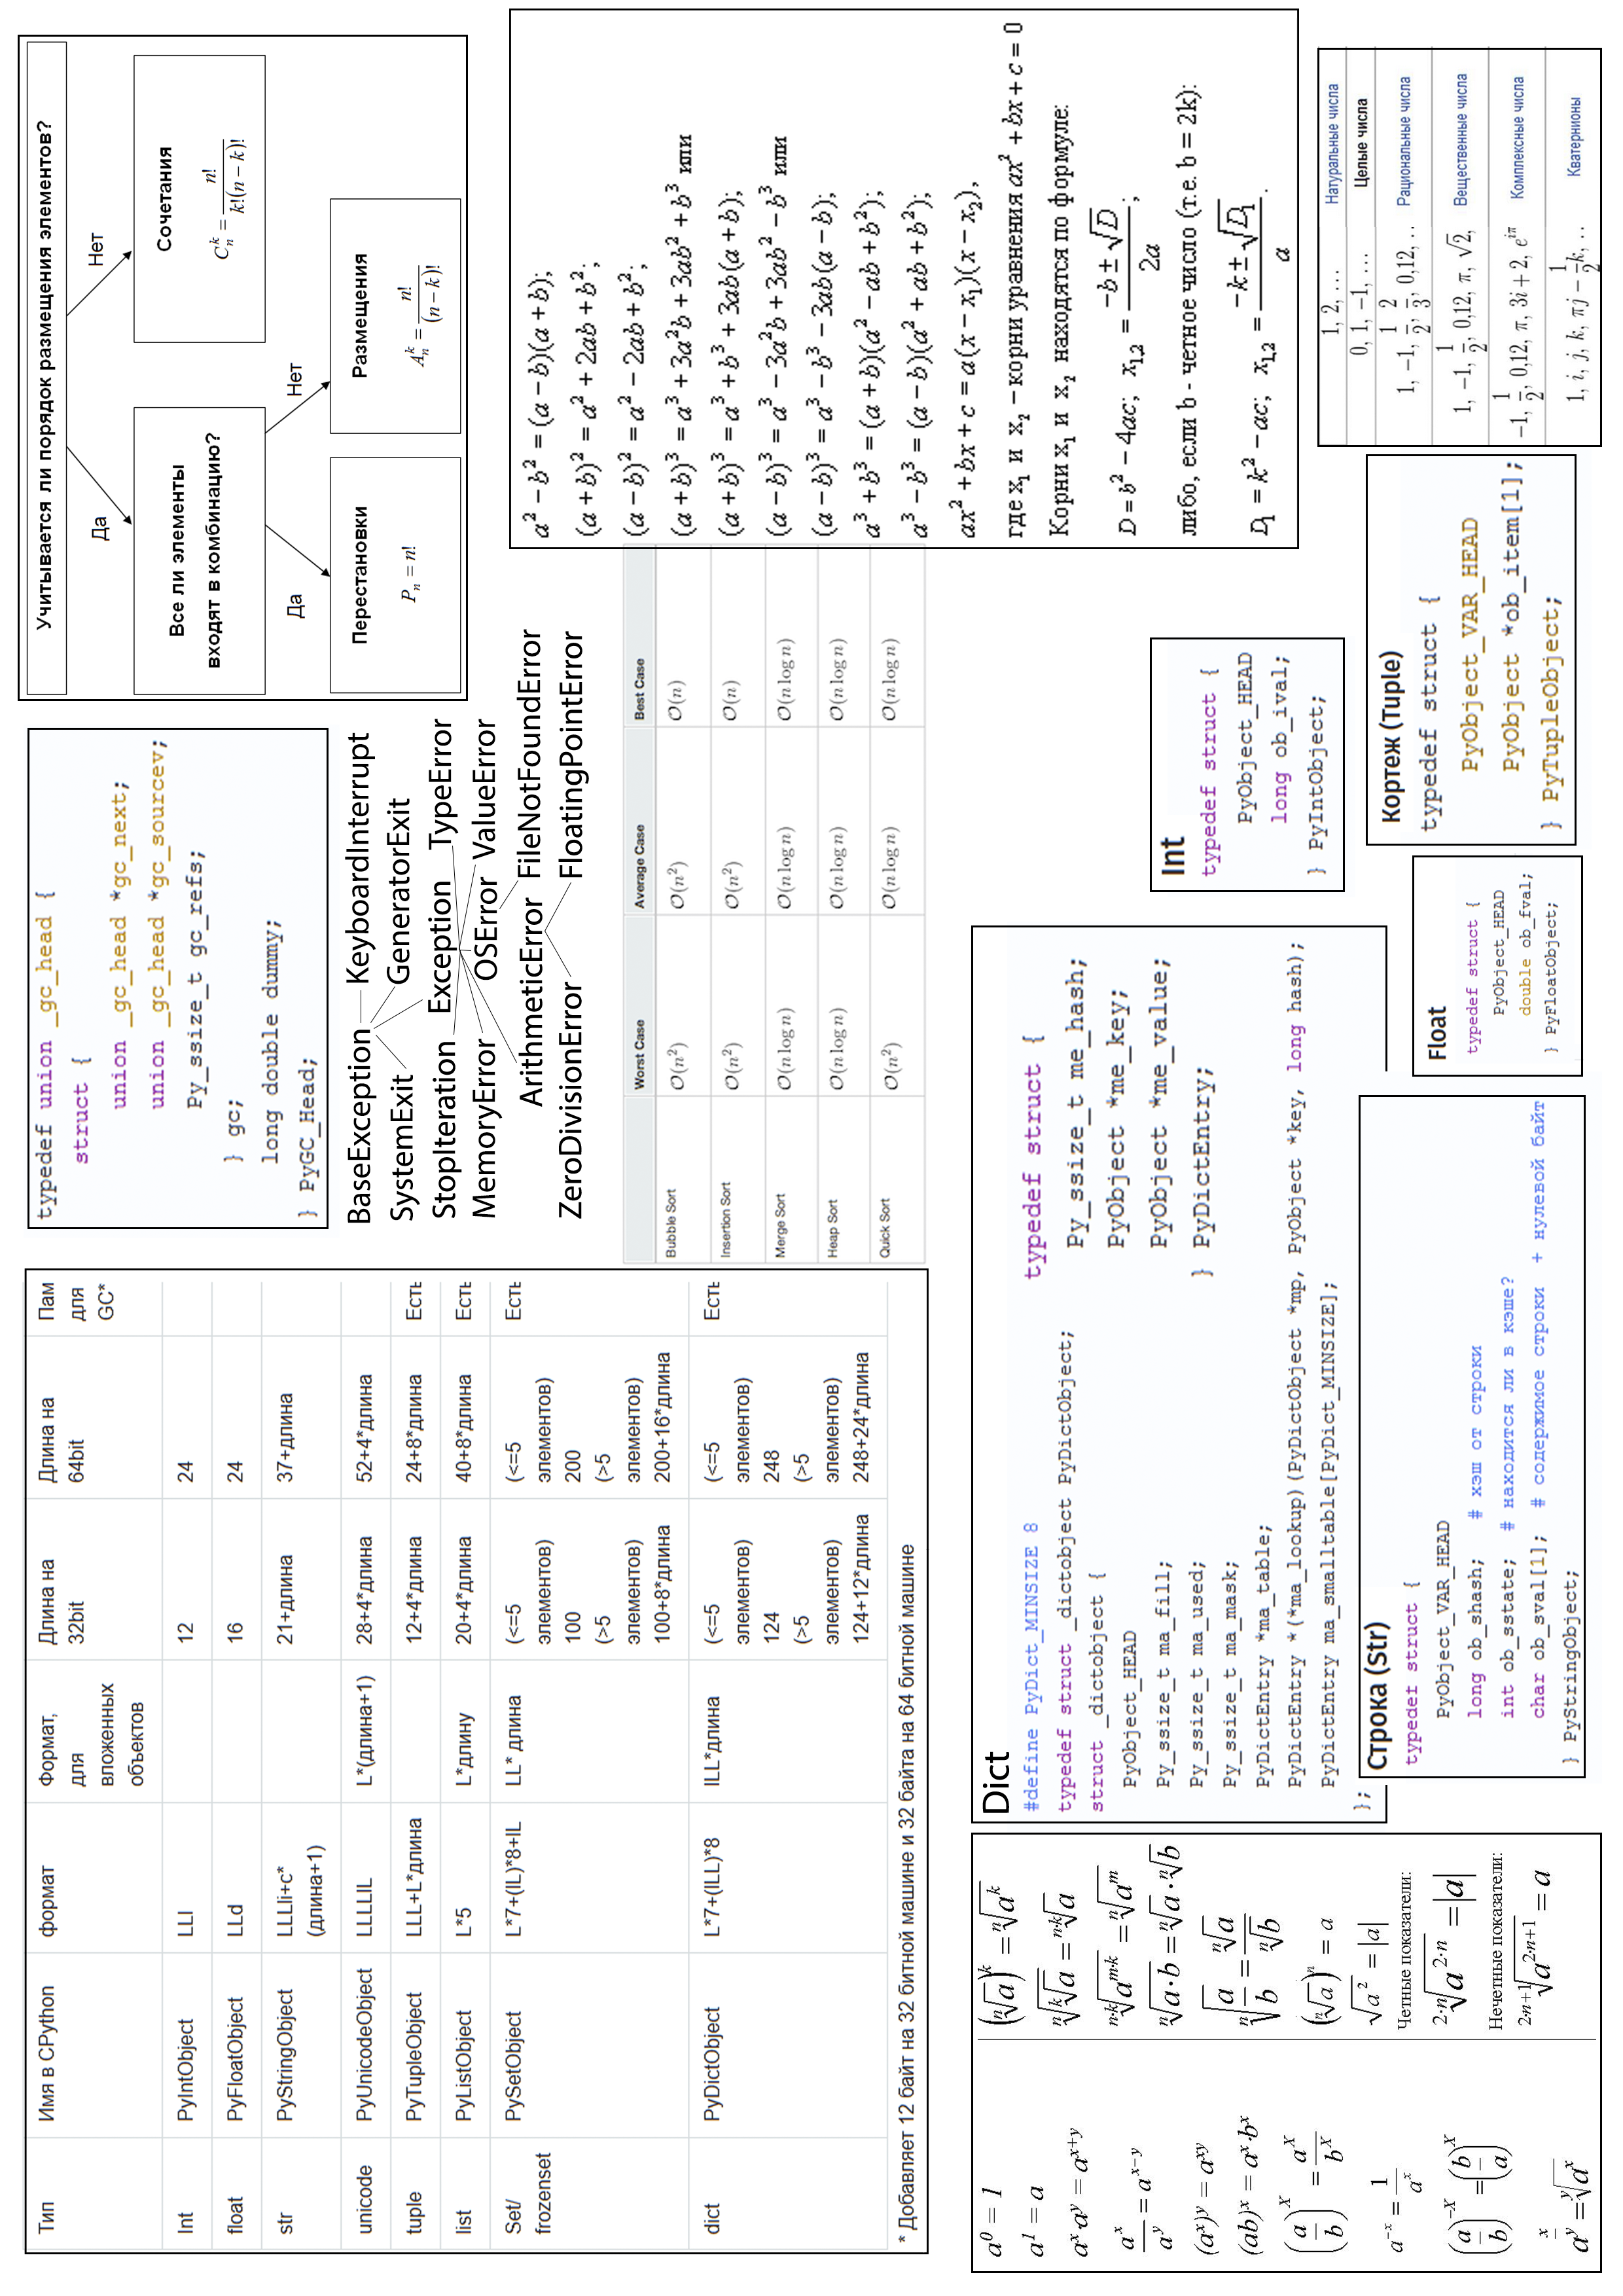
\includegraphics[width=\textwidth]{py_data_size.png}
\caption{Python usefull things}
\label{scheme}
\end{figure}

\section{Структуры базовых типов}

\section{GIL}

\subsection{Алгоритм работы}
\subsection{Эффективность переключения}

\section{Поколения сборщиков мусора}

\subsection{Алгоритм посчета ссылок}

\subsection{Отключение и ручной вызов GC2}

\chapter{Различные аспекты}

\section{Вызов в главной функции}
Что значит \pyth{if __name__=='__main__':}

Когда интерпретатор Python читает исходный файл, он исполняет весь найденный в нем код. Перед тем, как начать выполнять команды, он определяет несколько специальных переменных. Например, если интерпретатор запускает некоторый модуль (исходный файл) как основную программу, он присваивает специальной переменной \pyth{__name__} значение \pyth{"__main__"}. Если этот файл импортируется из другого модуля, переменной \pyth{__name__} будет присвоено имя этого модуля.

В случае с вашим сценарием, предположим, что код исполняется как основная функция, например:

\pyth{python threading_example.py}

После задания специальный переменных интерпретатор выполнит инструкцию import и загрузит указанные модули. Затем он проанализирует блок def, создаст объект-функцию и переменную под названием myfunction, которая будет указывать на этот объект.

Затем он прочтет инструкцию if, «поймёт», что \pyth{__name__} эквивалентен \pyth{"__main__"}, и выполнит указанный блок.

Одна из причин делать именно так – тот факт, что иногда вы пишете модуль (файл с расширением .py), предназначенный для непосредственного исполнения. Кроме того, он также может быть импортирован и использован из другого модуля. Производя подобную проверку, вы можете сделать так, что код будет исполняться только при условии, что данный модуль запущен как программа, и запретить исполнять его, если его хотят импортировать и использовать функции модуля отдельно.

Дополнительно см. \url{http://ibiblio.org/g2swap/byteofpython/read/module-name.html}.

\section{Импортирование модулей}
Что означает \pyth{threading_example} в данный момент импортируется из другого модуля?

Это означает, что кем-то в каком-либо файле .py (или в ходе интерактивной Python-сессии) используется выражение \pyth{import threading_example}. Противоположный этому случай – пользователь использует выражение \pyth{python threading_example.py} или \pyth{./threading_example.py}, и т. д.. В последнем случае, \pyth{threading_example.py} запущен как основная программа. В первом же случае он запущен как-то иначе (чтобы понять, ищите вызов вида \pyth{import threading_example}).

\section{Порядок вызова спец методов new, init, enter, exit, del}

Порядок вызова:

\begin{enumerate}
	\item \pyth{__new__()};
	\item \pyth{__init__()};
	\item \pyth{__enter__()}, если вызывается инструкция with;
	\item \pyth{__exit__()}, если вызывается инструкция with;
	\item \pyth{__del__()}
\end{enumerate}

\part{Реализация шаблонов (паттернов) проектирования}

\section{Сингелтон (Singleton)}

\linenumbers
\inputpython{singleton.py}{1}{100}
\nolinenumbers

\section{Adapter}

\section{Factory}

\section{Dependency}

\section{Injection}
